\documentclass[11pt,a4paper]{article}
\usepackage[T1]{fontenc}
\usepackage[utf8]{inputenc}
\usepackage{lmodern,microtype}
\usepackage{amsmath,amssymb,amsthm,mathtools,bm}
\usepackage{booktabs,array,tabularx,longtable}
\usepackage{graphicx,float,caption}
\usepackage{xcolor}
\usepackage[margin=20mm]{geometry}
\usepackage{enumitem,fancyhdr}
\usepackage[hidelinks]{hyperref}
\hypersetup{
 pdftitle={FIN ST94--ST105: Projection Uniqueness, Recovery, and Falsification},
 pdfauthor={Krzysztof Żuchowski},
 pdfsubject={Analytical and computational execution of FIN programs ST94--ST105},
 pdfkeywords={FIN, projection, conditional expectation, lift fiber, Petz recovery, Krawczyk, spin tower, identifiability, falsification}
}
\setlength{\parindent}{0pt}
\setlength{\parskip}{0.48em}
\setlength{\emergencystretch}{2em}
\setlength{\headheight}{14pt}
\setlist[itemize]{leftmargin=1.55em,itemsep=0.14em,topsep=0.2em}
\setlist[enumerate]{leftmargin=1.75em,itemsep=0.14em,topsep=0.2em}
\pagestyle{fancy}\fancyhf{}
\lhead{FIN ST94--ST105}\rhead{Release 10.62}\cfoot{\thepage}
\newtheorem{theorem}{Theorem}[section]
\newtheorem{proposition}[theorem]{Proposition}
\newtheorem{corollary}[theorem]{Corollary}
\newcommand{\proven}{\textcolor{green!40!black}{\textbf{[PROVEN]}}}
\newcommand{\strong}{\textcolor{blue!70!black}{\textbf{[STRONG EVIDENCE]}}}
\newcommand{\conditional}{\textcolor{violet!65!black}{\textbf{[CONDITIONAL]}}}
\newcommand{\openstatus}{\textcolor{red!72!black}{\textbf{[OPEN]}}}
\newcommand{\statusboundary}{\textcolor{orange!80!black}{\textbf{[BOUNDARY]}}}
\newcommand{\resultbox}[1]{\begin{center}\fcolorbox{blue!60!black}{blue!4}{\parbox{0.92\textwidth}{#1}}\end{center}}

\begin{document}
\pagenumbering{gobble}
\begin{titlepage}
\centering
\vspace*{1.1cm}
{\LARGE\bfseries FIN ST94--ST105\par}
\vspace{0.35cm}
{\Large Projection Uniqueness, Recovery, and Falsification\par}
\vspace{0.42cm}
{\large Conditional expectations, a complete 78-dimensional lift fiber, Petz recovery, state-dependent selection, passive realizations, an interval-certified fold, spin refinement, fine-observable identifiability, algebra towers, and a synthetic falsification protocol\par}
\vspace{0.95cm}
{\Large Krzysztof Żuchowski\par}
\vspace{0.24cm}
{\large Independent Researcher --- Fractal Information Theory Project\par}
{\large ORCID: 0009-0002-0909-3613\par}
\vspace{0.75cm}
{\large FIN Release 10.62 --- Version 1.0.0\par}
{\large August 11, 2026\par}
\vfill
\begin{minipage}{0.90\textwidth}
\textbf{Research question.} Can the exact projection fiber found in ST86 be made unique, recoverable, and falsifiable without silently inserting the observable algebra, selector, clock, scale, or apparatus?\par
\textbf{Method.} Finite $C^*$-algebra conditional expectations, exact block-operator classification, quantum relative entropy and Petz sufficiency, equivariant dynamics, passive realization theory, outward interval arithmetic, covering-space holonomy, Fisher/Chernoff information, and twenty-eight live tests.\par
\textbf{Epistemic rule.} The hypothesis that observable reality is a projection of FIN remains counterfactual. The report distinguishes a unique map after an observable algebra is supplied from a strict theorem selecting that algebra.\par
\textbf{Repository snapshot.} Git commit \texttt{dc6f8f924d1636af284f386d145103eb694c2034}; additional local artifacts are listed in the release manifest.\par
\textbf{Repository.} \url{https://github.com/hyconiek/Fractal-Nadsoliton-Theory}\par
\textbf{License.} CC BY 4.0.
\end{minipage}
\end{titlepage}
\pagenumbering{arabic}

\begin{abstract}
ST94--ST105 turn the projection interpretation of FIN into a sharper mathematical program. ST94 proves that once a unital observable algebra $\mathcal B$ and normalized trace are supplied, the trace-preserving conditional expectation onto $\mathcal B$ is unique. For the coarse/fine split the natural algebra is $M_{12}\oplus\mathbb C$. This is relative uniqueness: strict $A$ still does not select the observable algebra or the apparatus realizing it.

ST95 classifies every real symmetric graph Laplacian $L$ on 24 vertices satisfying $LP=PA_{12}$. In the plus/minus basis,
\[
L=P A_{12}P^*+F B F^*,
\]
where $B$ ranges over a 78-dimensional convex spectrahedral set. Positivity requires $B\succeq0$; the graph-sign constraints are $B_{ii}\ge A_{ii}$ and $A_{ij}\le B_{ij}\le-A_{ij}$ for $i\ne j$. The former one-parameter family $A_{24}(q)$ occupies only a tiny subfamily. The exact nonidentifiability discovered in ST86 is therefore much larger than previously shown.

ST96 gives the exact Petz-recovery boundary. For spectral pinching $\Pi$ and a faithful reference state in its range,
\[
D(\rho\|\sigma)=D(\rho\|\Pi\rho)+D(\Pi\rho\|\sigma).
\]
Recovery is exact precisely when no coarse/fine coherence was discarded. ST97 constructs a state-dependent twelve-branch selector, but proves that the symmetric state remains fixed and nonselecting; initial phase merely relocates the missing premise. ST98 extends the passive-memory no-go to reciprocal state-space realizations.

ST99 closes the first fold obligation for the frozen binary64 strict operator. A 15-variable Krawczyk calculation gives strict inclusion with margin $9.9999871\times10^{-9}$ in a radius-$10^{-8}$ box. This is a source-code interval theorem for the frozen numerical operator, not yet a transcendental-parameter certificate. ST100 proves that a degree-two refinement squares $\mathbb Z_2$ holonomy, so an antiperiodic spin class becomes periodic; maintaining antiperiodicity requires a new twist at every level.

ST101 proves that one deliberately fine/global scalar observable identifies the hidden dyadic parameter. The fine block satisfies $B(q)=B(0)+2qI$, and the globally normalized Gibbs coarse-sector probability is strictly monotone in $q$. ST102 constructs a commuting conditional-expectation tower. ST103 proves the common-contamination endpoint by data processing but leaves the independent nuisance rectangle uncertified. ST104 proves $\mathrm{TO}\subseteq\mathrm{CGP}\subsetneq\mathrm{GP}$ and keeps the first strictness question open. ST105 proves that conditioned coarse records cannot distinguish $q_0$ from $q_1$, while a supplied coarse/fine occupation measurement can do so synthetically. Projection is now mathematically precise and conditionally falsifiable, but it remains unselected and experimentally untested.
\end{abstract}

\textbf{Status vocabulary.} \proven{} denotes an exact analytic, finite, or source-code interval result in its stated scope. \strong{} denotes stable numerical evidence. \conditional{} means that displayed additional resources are required. \openstatus{} marks an attempted target not closed. \statusboundary{} records a non-implication.

\tableofcontents
\newpage

\section{Frozen object, kernel discipline, and target}

The strict working operator remains
\begin{equation}
W_{xx}=0,\qquad W_{xy}=\frac{\cos(0.18575d(x,y)+0.16250)}{1+d(x,y)^{1.8}}\quad(x\ne y),
\qquad A=sI-W,
\label{eq:strict}
\end{equation}
on $C_{12}$, with $s=1.660307278766099$ to the displayed precision. Therefore
\[
\langle f,Af\rangle=\frac12\sum_{x,y}W_{xy}|f_x-f_y|^2\ge0.
\]
The zero diagonal is explicit. The legacy ontological kernel remains an intermediate bridge kernel. This report neither identifies it with~\eqref{eq:strict} nor transfers its physical roles.

The ST86 isometries are
\[
P=\frac1{\sqrt2}\begin{pmatrix}I\\I\end{pmatrix},\qquad
F=\frac1{\sqrt2}\begin{pmatrix}I\\-I\end{pmatrix},
\qquad P^*P=F^*F=I,\quad P^*F=0.
\]
ST86 proved $P^*f(A_{24}(q))P=f(A)$ for every fixed finite spectral function $f$. ST94--ST105 ask:
\begin{enumerate}
\item Is the projection map unique without assuming its target algebra?
\item How large is the complete fiber of deeper graph generators?
\item Which lost states are exactly recoverable?
\item Can a state generate a canonical selector?
\item Can active time emerge from a wider passive realization?
\item Can the nonlinear fold be interval-certified?
\item How do spin classes behave under refinement?
\item What is the smallest observable that destroys coarse nonidentifiability?
\end{enumerate}

\resultbox{\textbf{Principal conclusion.} Once the observable algebra is supplied, the trace-preserving projection is unique. Strict FIN does not supply that algebra. The deeper graph-generator fiber is 78-dimensional, exact recovery is limited to block-diagonal states, and one deliberately fine/global measurement restores identifiability. Thus projection becomes a sharp conditional model, not a derived physical ontology.}

\section{Outcome matrix}
\small
\begin{longtable}{@{}p{0.06\textwidth}p{0.29\textwidth}p{0.25\textwidth}p{0.31\textwidth}@{}}
\toprule ID & Object & Result & Boundary\\\midrule\endfirsthead
\toprule ID & Object & Result & Boundary\\\midrule\endhead
ST94 & Conditional expectation & \proven{} relative uniqueness & Observable algebra remains supplied\\
ST95 & Complete lift fiber & \proven{} 78-dimensional classification & No physical refinement law\\
ST96 & Petz recovery & \proven{} exact equality frontier & Pinching/reference supplied\\
ST97 & State-dependent selector & \proven{} constructed mechanism & Symmetric state and QW-2191 remain\\
ST98 & Passive realization & \proven{} extended no-go & Active/antisymmetric source lies outside\\
ST99 & Fold certificate & \proven{} for frozen binary64 $A$ & No transcendental-kernel enclosure\\
ST100 & Spin tower & \proven{} pullback classification & New twists are unselected\\
ST101 & Fine identifiability & \proven{} conditional one-scalar theorem & Measurement and $\beta$ supplied\\
ST102 & Algebra tower & \proven{} commuting expectations & Coherence does not select fine blocks\\
ST103 & Robust nuisance & \proven{} common diagonal; \openstatus{} full box & Independent max--min uncertified\\
ST104 & Thermal hierarchy & \proven{} right strict inclusion & Bath-dependent left strictness open\\
ST105 & Projection protocol & \proven{} coarse impossibility; \strong{} fine counts & Entire protocol synthetic\\
\bottomrule
\end{longtable}
\normalsize

\section{ST94: what does and does not make a projection unique}

Let $P_c=PP^*$ and $P_f=FF^*$. Suppose the operationally accessible algebra has already been declared to be
\[
\mathcal B=P M_{12}P^*\oplus\mathbb C P_f.
\]
Define
\begin{equation}
E_{\mathcal B}(X)=P_cXP_c+\frac{\operatorname{Tr}(P_fXP_f)}{12}P_f.
\label{eq:expectation}
\end{equation}

\begin{theorem}[Relative uniqueness]
For a fixed unital finite-dimensional $*$-subalgebra $\mathcal B\subset M_n$ and normalized trace $\tau$, there is exactly one $\tau$-preserving conditional expectation $E_{\mathcal B}:M_n\to\mathcal B$. For the displayed coarse/fine algebra it is~\eqref{eq:expectation}.
\end{theorem}

\textit{Proof.} The bimodule and trace identities imply
\[
\tau\bigl(B^*(X-E_{\mathcal B}X)\bigr)=0\qquad(B\in\mathcal B).
\]
Thus $E_{\mathcal B}$ is the Hilbert--Schmidt orthogonal projection onto $\mathcal B$, which is unique. Direct block evaluation gives~\eqref{eq:expectation}. \hfill$\square$

Live tests verify unitality, trace preservation, idempotence and the bimodule identity with residuals below $2.0\times10^{-13}$.

The theorem identifies the exact location of the missing axiom. ``Operational sufficiency'' does not derive the observable algebra; it only makes the expectation unique after that algebra is fixed. Many other subalgebras, bases and accessible-sector declarations remain mathematically possible. Consequently ST94 does not turn the projected-universe hypothesis into a strict theorem.

\section{ST95: complete classification of the hidden lift fiber}

Let $L=L^*$ satisfy $LP=PA$. Self-adjointness makes $P\mathbb R^{12}$ reducing, so the most general form is
\begin{equation}
L=PAP^*+FBF^*,\qquad B=B^*.
\label{eq:fiber}
\end{equation}
In the original two-layer basis,
\[
L=\frac12\begin{pmatrix}A+B&A-B\\A-B&A+B\end{pmatrix}.
\]

\begin{theorem}[Complete graph-lift fiber]
The matrix~\eqref{eq:fiber} is positive semidefinite iff $B\succeq0$. It is a graph Laplacian with nonpositive off-diagonal entries iff
\begin{equation}
B_{ii}\ge A_{ii},\qquad A_{ij}\le B_{ij}\le-A_{ij}\quad(i\ne j).
\label{eq:graphfiber}
\end{equation}
The admissible set has full affine dimension $12\cdot13/2=78$.
\end{theorem}

\textit{Proof.} The $(P,F)$ basis diagonalizes $L$ into $A\oplus B$, proving the PSD statement. Reading the within-layer, cross-layer and paired cross-layer off-diagonal entries gives~\eqref{eq:graphfiber}. The vector of all ones lies in the coarse sector and is annihilated by $A$, so every admissible $L$ has zero row sum. Finally, $B=cI$ with $c>\max_iA_{ii}$ is positive definite and satisfies every inequality strictly because all strict weights are positive. Hence the set has nonempty interior in the 78-dimensional symmetric-matrix space. \hfill$\square$

\begin{figure}[H]\centering
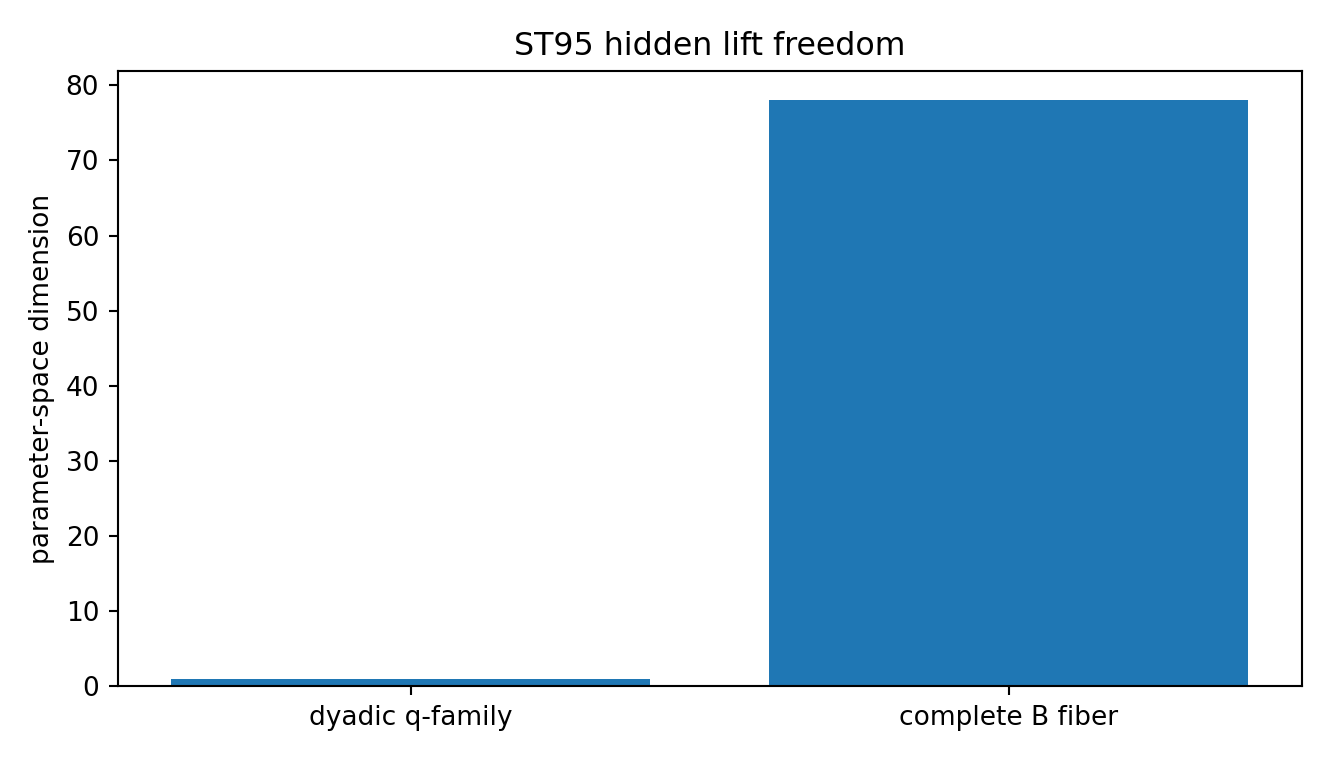
\includegraphics[width=0.67\textwidth]{FIN_ST94_ST105_Figures/st95_lift_dimension.png}
\caption{The one-parameter dyadic family is a negligible slice of the complete 78-dimensional coarse-preserving graph-lift fiber.}
\end{figure}

This is stronger than ST86. The invisible freedom is not merely one unknown $q$; it is an entire convex spectrahedral family. Any claim that coarse FIN dynamics uniquely reconstructs a deeper universe is therefore false without substantially stronger locality, action, naturality, or observational premises.

\section{ST96: exact recovery and the shape of lost information}

Let
\[
\Pi(X)=P_cXP_c+P_fXP_f
\]
be coarse/fine pinching. If a faithful reference state $\sigma$ lies in the pinched algebra, conditional-expectation sufficiency gives
\begin{equation}
D(\rho\|\sigma)=D(\rho\|\Pi\rho)+D(\Pi\rho\|\sigma).
\label{eq:pythagoras}
\end{equation}

\begin{theorem}[Petz frontier]
The Petz recovery map recovers $\Pi\rho$. It recovers $\rho$ itself iff
\[
\rho=\Pi\rho,
\]
equivalently iff every coarse/fine coherence block vanishes. Moreover
\[
D(\rho\|\Pi\rho)\ge\frac12\|\rho-\Pi\rho\|_1^2.
\]
\end{theorem}

Sixteen random faithful states verify~\eqref{eq:pythagoras} to $5.0\times10^{-16}$; every sampled Pinsker margin is positive.

\begin{figure}[H]\centering
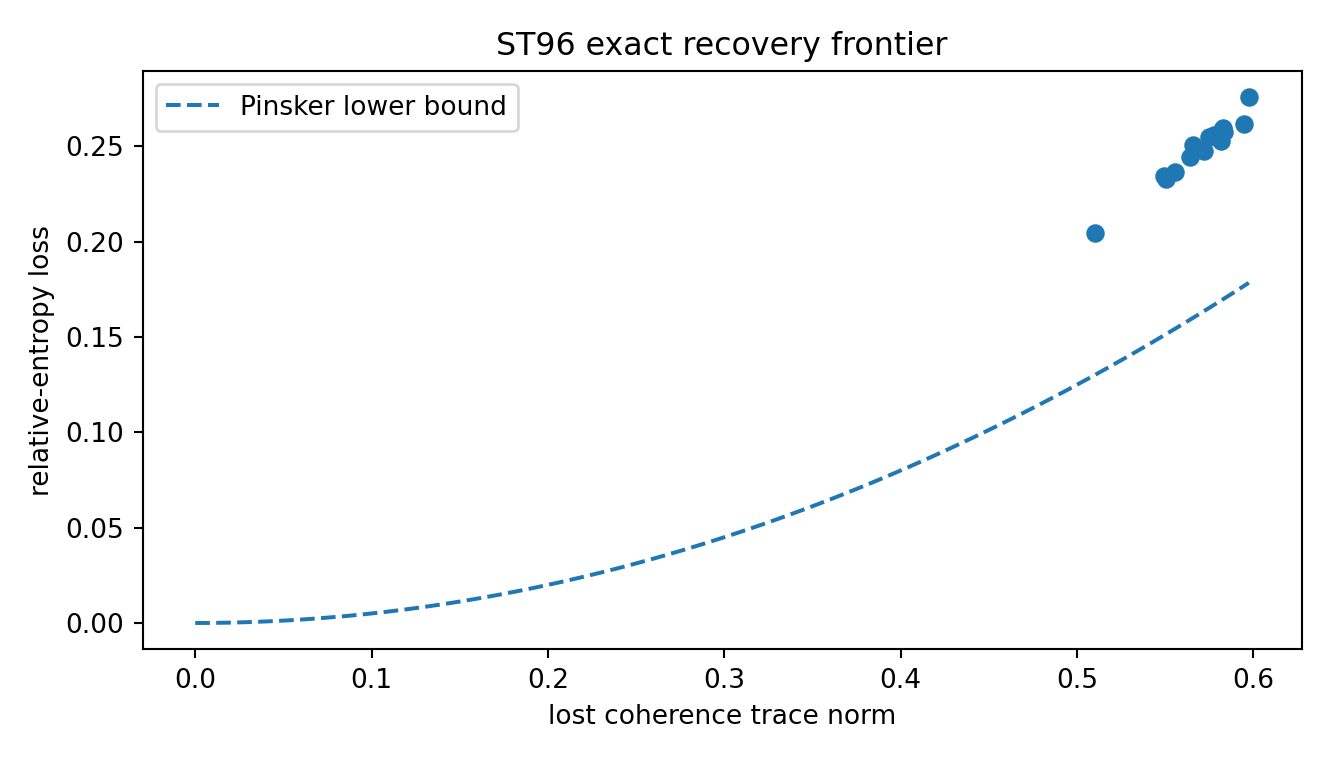
\includegraphics[width=0.70\textwidth]{FIN_ST94_ST105_Figures/st96_recovery.png}
\caption{Relative-entropy loss versus discarded coherence. The dashed curve is the Pinsker lower bound.}
\end{figure}

The result converts a vague ``projection loses information'' statement into an exact criterion. Within-block information is recoverable; cross-block coherence is not. This criterion is relative to the supplied $\Pi$ and $\sigma$ and does not prove a physical measurement process.

\section{ST97--ST98: selection and time do not emerge for free}

\subsection{A state-dependent selector}

Consider the constructed equivariant normal form
\[
\dot r=r(\mu-r^2),\qquad \dot\theta=-g\sin(12\theta),\qquad \mu,g>0.
\]
It has twelve stable angular branches $\theta=k\pi/6$ and twelve unstable separatrices. The sampled nonzero initial states reach all twelve stable branches.

\begin{proposition}[Relocation, not elimination, of selection]
Every nonzero state outside the unstable separatrices selects a branch through its initial phase. The symmetric state $r=0$ remains invariant and selects nothing. Reflection maps a selected branch to its reflected partner.
\end{proposition}

\begin{figure}[H]\centering
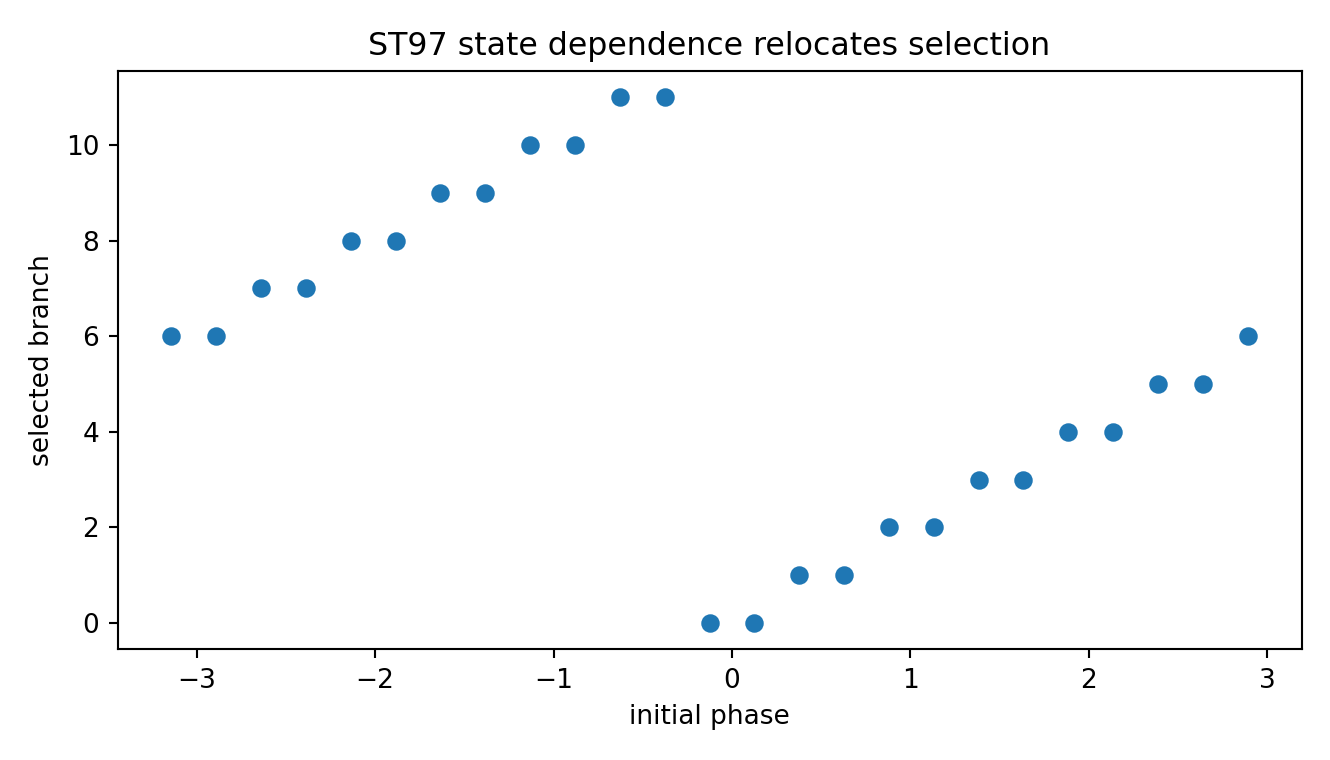
\includegraphics[width=0.70\textwidth]{FIN_ST94_ST105_Figures/st97_state_selector.png}
\caption{Initial phase determines the branch in the constructed equivariant flow. This demonstrates state-dependent selection while exposing its initial-condition premise.}
\end{figure}

The user's idea that symmetry provides a reservoir of possible realizations is mathematically sound. Symmetry is not itself positive feedback. The instability and nonlinear angular law amplify a supplied perturbation. QW-2191 remains open because strict $A$ neither supplies that law nor chooses the initial phase.

\subsection{A wider passive-memory no-go}

ST98 replaces a scalar Stieltjes sum by a reciprocal state-space realization
\[
M(z)=B^*(zI+C)^{-1}B,\qquad C=C^*>0.
\]
Diagonalizing $C$ shows that all poles lie in the stable half-plane and every residue matrix is $b_j^*b_j\succeq0$. Hence $M$ is positive real and passive. If $C$ and $B$ are constructed only from commuting real functions of strict $A$, neither an antisymmetric orientation nor a signed active residue appears.

\begin{figure}[H]\centering
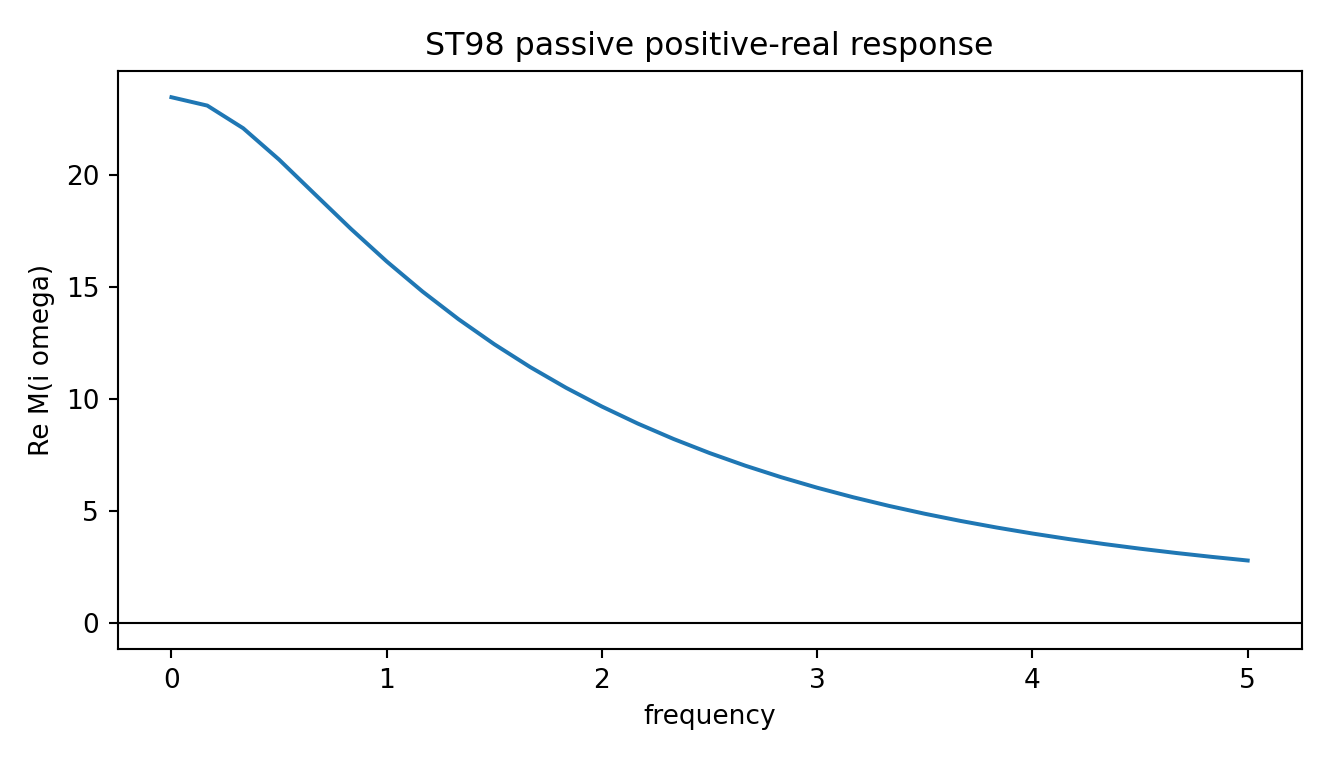
\includegraphics[width=0.70\textwidth]{FIN_ST94_ST105_Figures/st98_passive_response.png}
\caption{Positive real part of a sampled reciprocal realization. The plotted calculation illustrates the analytic residue theorem.}
\end{figure}

Active temporal gain therefore requires a genuinely new source class: an indefinite metric, pump, antisymmetric coupling, or nonequilibrium state. Passive memory can encode history without generating a physical arrow of time.

\section{ST99: interval closure of the first nonlinear fold}

The reflection-reduced fold system has 15 variables:
\[
G(q,\kappa,v)=
\begin{pmatrix}
g(q,\kappa)\\H(q,\kappa)v\\(\|v\|^2-1)/2
\end{pmatrix}=0.
\]
ST99 evaluates the rational saturation terms and the complete Jacobian with 70-digit outward interval arithmetic. The approximate inverse is used only as a Krawczyk preconditioner. For the radius-$10^{-8}$ box around the ST83 center,
\[
K(X)\subset\operatorname{int}(X),\qquad
\min_i\operatorname{dist}(K_i(X),\partial X_i)
=9.999987060638205\times10^{-9}.
\]
The maximum Krawczyk half-width is $1.25\times10^{-14}$. Five smaller boxes also pass.

\begin{theorem}[Frozen-operator fold certificate]
For the exact frozen binary64 matrix $A$ used by the local scripts, the 15-variable fold system has one unique zero in the certified radius-$10^{-8}$ box centered at
\[
\kappa=0.016589052386382905.
\]
\end{theorem}

\begin{figure}[H]\centering
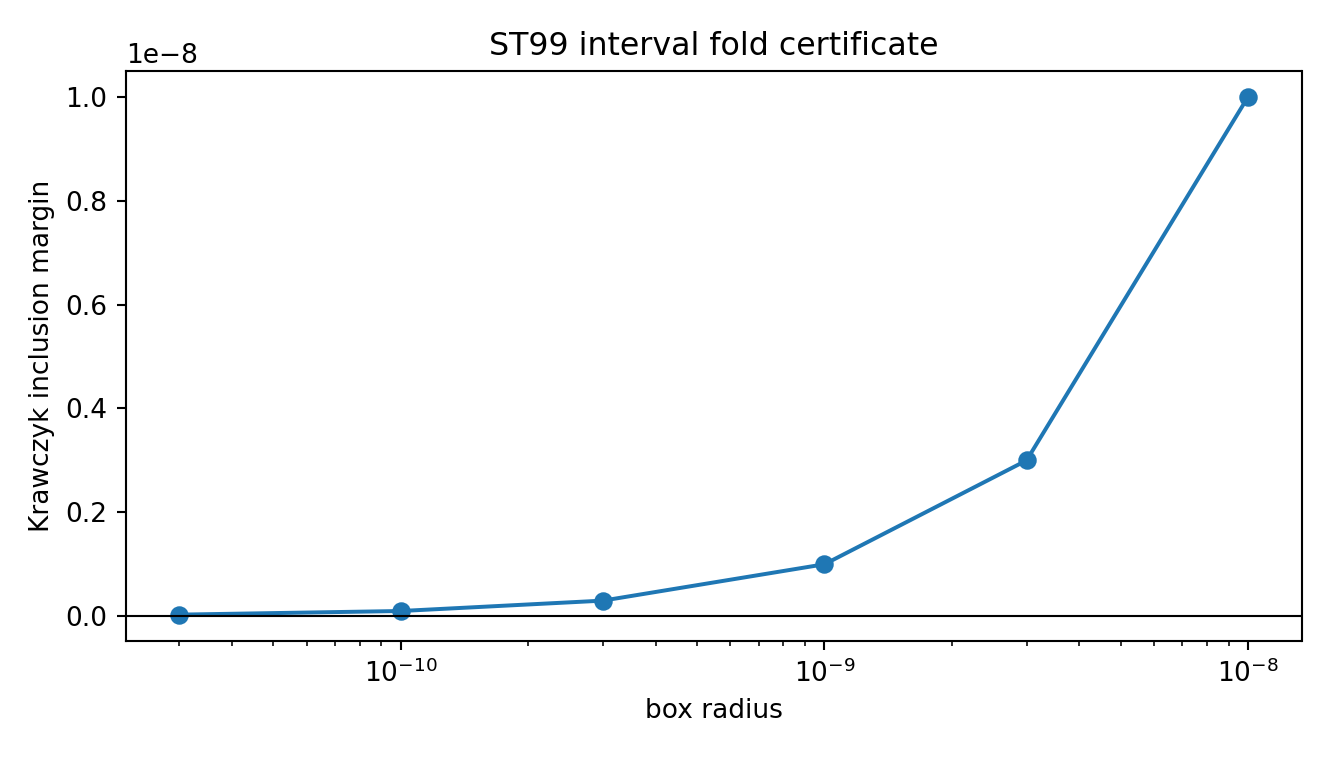
\includegraphics[width=0.70\textwidth]{FIN_ST94_ST105_Figures/st99_krawczyk.png}
\caption{Every attempted box has positive strict Krawczyk inclusion margin.}
\end{figure}

This promotes the local simple fold from strong floating evidence to a source-code interval theorem in its declared scope. It does not enclose the transcendental construction of $A$ from cosine and $d^{9/5}$, prove a branch connection to $\kappa=1$, or establish stability.

\section{ST100: spin holonomy under refinement}

A degree-two cover of circles maps the generator of the fine fundamental group to twice the coarse generator. For a $\mathbb Z_2$ holonomy $h\in\{+1,-1\}$,
\[
h_{\rm fine}=h_{\rm coarse}^2=+1.
\]
Thus the only pullback sequences through $12\to24\to48$ are
\[
(+1,+1,+1),\qquad(-1,+1,+1).
\]

\begin{corollary}[New-twist obligation]
There is no stationary antiperiodic pullback sequence. Keeping $h=-1$ at every refinement requires inserting a new twist class at every level.
\end{corollary}

The result is a new obstruction to interpreting the $C_{24}$ cover as an automatically scale-consistent spin source. Projective structure exists, but refinement does not propagate it in the desired nontrivial class without additional boundary data.

\section{ST101--ST102: the smallest visible crack in the projection}

\subsection{One scalar fine observable identifies the dyadic parameter}

For the dyadic family the hidden block is especially simple:
\begin{equation}
B(q)=B(0)+2qI.
\label{eq:qshift}
\end{equation}
Therefore one calibrated fine-sector expectation of the generator determines $q$. An alternative uses the normalized Gibbs ensemble. Let
\[
Z_c=\operatorname{Tr}e^{-\beta A},\qquad Z_{f0}=\operatorname{Tr}e^{-\beta B(0)}.
\]
Then the probability of occupying the coarse sector is
\begin{equation}
p_c(q)=\frac{Z_c}{Z_c+e^{-2\beta q}Z_{f0}},
\qquad
q=-\frac1{2\beta}\log\left(\frac{1-p_c}{p_c}\frac{Z_c}{Z_{f0}}\right).
\label{eq:qrecover}
\end{equation}

\begin{figure}[H]\centering
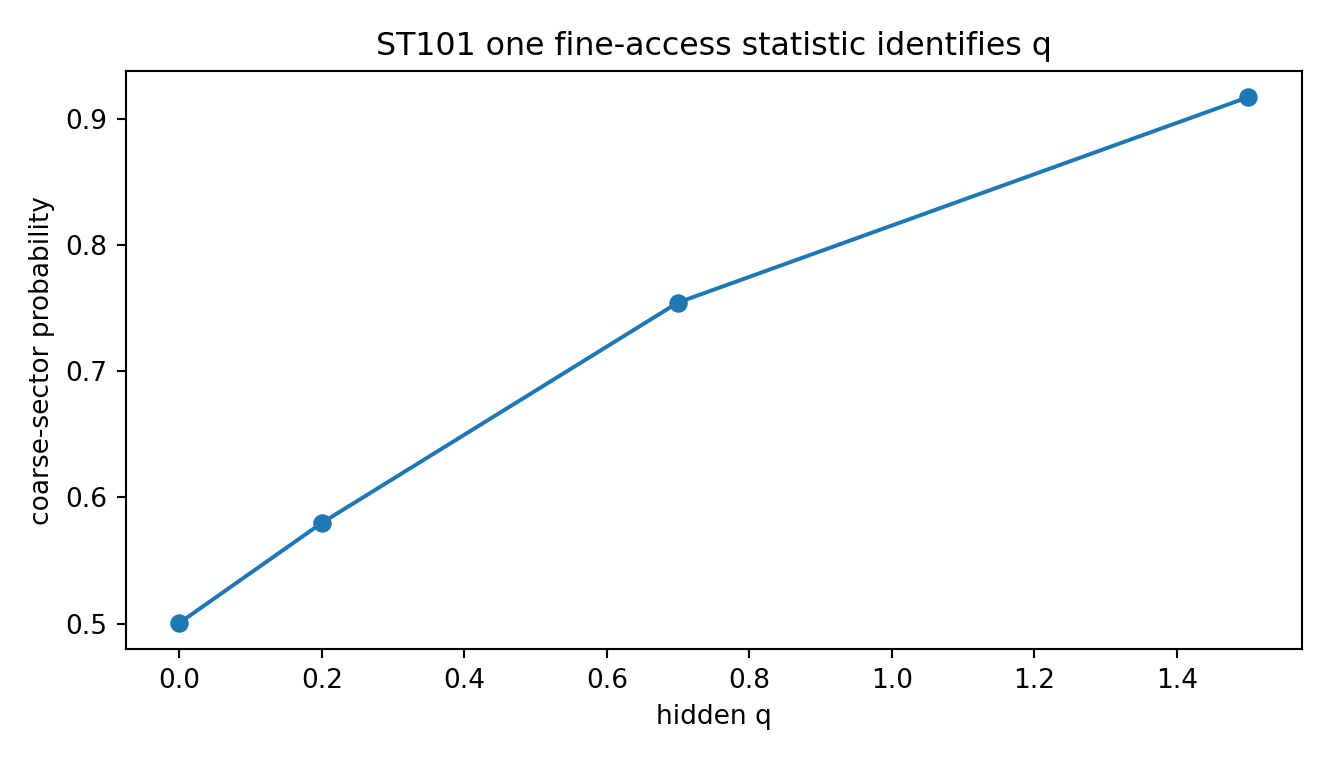
\includegraphics[width=0.70\textwidth]{FIN_ST94_ST105_Figures/st101_identifiability.png}
\caption{The globally normalized coarse-sector probability is strictly monotone in the hidden dyadic parameter.}
\end{figure}

This resolves the Gibbs normalization caveat from ST86. Conditioned coarse states remain identical, but the global coarse-sector occupation is fine-sensitive. The bridge is conditional on $\beta$, global preparation, baseline partition functions and a calibrated coarse/fine measurement.

\subsection{Commuting expectation tower}

On 48 sites, let $E_{24}$ average over the half-translation subgroup and let $E_{12}$ average over the order-four subgroup generated by translation by 12. These finite group averages are trace-preserving conditional expectations. Since the groups are nested and abelian,
\[
E_{24}E_{12}=E_{12}E_{24}=E_{12}.
\]
The composite isometry also satisfies
\[
A_{48}P_{24}P_{12}=P_{24}P_{12}A_{12}
\]
for arbitrary intermediate fine parameters. Live residuals are below $2.7\times10^{-15}$. This is a genuine commuting-square tower, but its coherence is automatic and selects no hidden block or physical renormalization law.

\section{ST103--ST104: statistical and thermodynamic boundaries}

\subsection{What can be certified about nuisance contamination}

For common contamination
\[
p_\epsilon=(1-\epsilon)p+\epsilon u,\qquad
q_\epsilon=(1-\epsilon)q+\epsilon u,
\]
increasing $\epsilon$ is application of the same stochastic channel to both hypotheses. Chernoff information cannot increase under a common channel. The exact worst endpoint on $0\le\epsilon\le0.12$ is therefore $\epsilon=0.12$, with deterministic numerical value $0.0404022886255$ nats/event for the frozen synthetic tables.

\begin{figure}[H]\centering
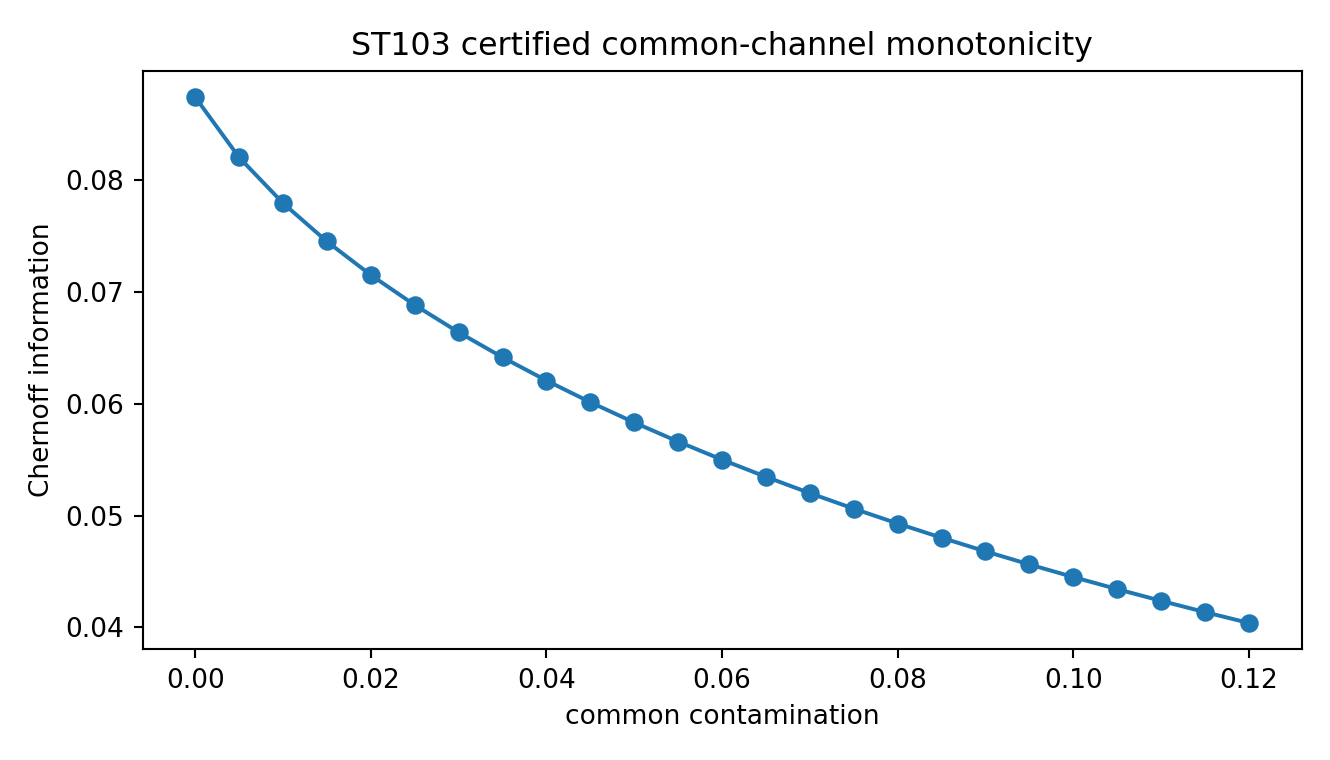
\includegraphics[width=0.70\textwidth]{FIN_ST94_ST105_Figures/st103_common_nuisance.png}
\caption{The sampled curve illustrates the exact data-processing monotonicity theorem on the common-contamination diagonal.}
\end{figure}

The full ST103 target remains open. Independent $\epsilon_P$ and $\epsilon_Q$ do not arise from one common channel, and this batch obtains no outward global max--min certificate over that rectangle. The ST87 boundary optimum remains strong numerical evidence.

\subsection{Thermal-operation hierarchy}

The strict spectral multiplicities are $(1,2,2,2,2,2,1)$, so the zero-Bohr-frequency operator sector has dimension
\[
1^2+5\cdot2^2+1^2=22.
\]
Energy-conserving thermal operations are covariant and Gibbs preserving:
\[
\mathrm{TO}\subseteq\mathrm{CGP}\subseteq\mathrm{GP}.
\]
ST89's coherence-creating measure-and-prepare channel proves
\[
\mathrm{CGP}\subsetneq\mathrm{GP}.
\]
Whether $\mathrm{TO}\subsetneq\mathrm{CGP}$ for the exact declared spectrum depends on a bath/dilation definition not supplied by FIN and remains open. Degeneracy allows zero-frequency coherence within equal-energy blocks; it does not generate a bath or dimensionful Hamiltonian.

\section{ST105: a projection-specific falsification protocol}

Choose the synthetic alternatives
\[
H_0:q=0.2,\qquad H_1:q=0.7,\qquad\beta=0.8.
\]
Every record confined to the conditioned coarse functional calculus has identical distributions, hence total variation zero and optimal equal-prior error $1/2$ for every sample size. The global coarse/fine Gibbs occupation from~\eqref{eq:qrecover} has probabilities
\[
p_0=0.5797389466,\qquad p_1=0.7543042531.
\]
For $n$ independent binary events the exact likelihood formula is binomial. Its binary64 evaluation first falls below $1\%$ Bayes error at $n=154$.

\begin{figure}[H]\centering
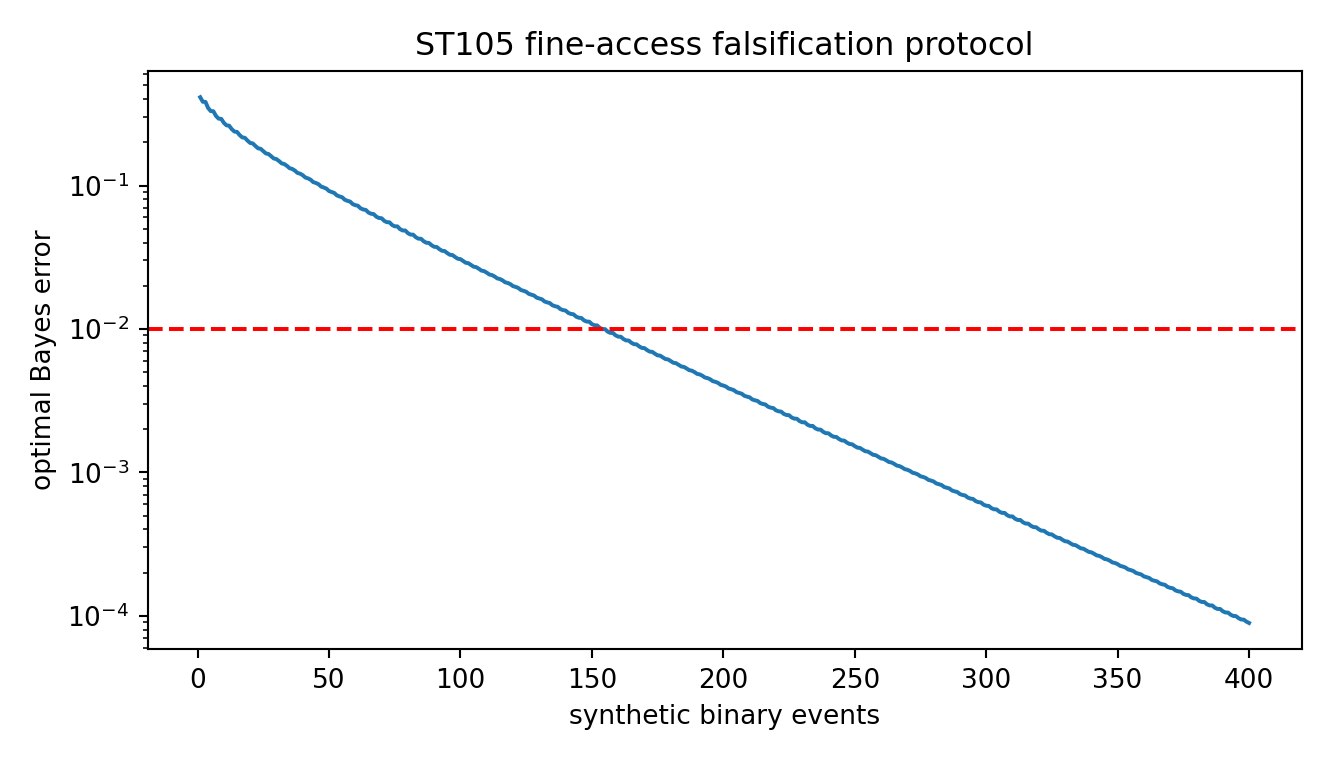
\includegraphics[width=0.70\textwidth]{FIN_ST94_ST105_Figures/st105_falsification.png}
\caption{Synthetic optimal equal-prior error after adding deliberately fine/global access. The event count is not a laboratory recommendation.}
\end{figure}

The protocol supplies a clean logical falsifier: if two proposed hidden lifts predict different globally normalized coarse/fine occupation, one binary measurement class can distinguish them. But FIN does not supply a global Gibbs preparation, physical $\beta$, coarse/fine POVM, detector, custody or independent events. The result is an executable specification, not experimental evidence.

\section{Falsification ledger}

\begin{longtable}{@{}p{0.30\textwidth}p{0.18\textwidth}p{0.44\textwidth}@{}}
\toprule Claim & Verdict & Reason\\\midrule\endfirsthead
\toprule Claim & Verdict & Reason\\\midrule\endhead
Operational sufficiency uniquely selects a projection & False as stated & It uniquely fixes $E_{\mathcal B}$ only after $\mathcal B$ is supplied\\
The dyadic $q$ family exhausts deeper lifts & Refuted & Complete graph-lift fiber has dimension 78\\
All projected information is recoverable & Refuted & Cross-sector coherence is lost exactly by ST96\\
A state-dependent law removes the selector premise & Refuted in construction & Initial phase/boundary data carry the choice\\
Reciprocal passive memory creates active time & Refuted in class & Positive-real realization theorem\\
The first localized fold is a numerical artifact & Refuted for frozen $A$ & Strict Krawczyk inclusion proves a unique fold root locally\\
Antiperiodic spin automatically persists across scales & Refuted & Degree-two pullback squares holonomy to $+1$\\
Hidden $q$ is absolutely unobservable & Refuted conditionally & One fine/global scalar identifies it\\
Refinement coherence selects the hidden dynamics & Refuted & Commuting square is automatic for all fine parameters\\
ST103 fully certifies independent nuisance & Not achieved & Only common-channel diagonal is proved\\
Gibbs preservation equals thermal operation & Refuted & ST89 violates covariance\\
Projection is experimentally supported & Not established & All carriers, preparations and events remain synthetic\\
\bottomrule
\end{longtable}

\section{Recommended programs ST106--ST117}

\begin{enumerate}
\item[\textbf{ST106}] Classify additional naturality/locality axioms that might select the observable algebra without assuming it.
\item[\textbf{ST107}] Derive extreme rays, faces and boundary dimensions of the 78-dimensional graph-lift spectrahedron.
\item[\textbf{ST108}] Enclose the transcendental kernel entries and lift ST99 beyond the frozen binary64 operator.
\item[\textbf{ST109}] Test Petz sufficiency for several noncommuting reference states and find the maximal recoverable code.
\item[\textbf{ST110}] Seek a strict-derived nonzero initial-state measure or prove equivariant-measure nonselection.
\item[\textbf{ST111}] Classify active memory realizations with one antisymmetric block and audit every new source premise.
\item[\textbf{ST112}] Optimize Fisher/Chernoff design for $q$ under finite $\beta$ and detector nuisance.
\item[\textbf{ST113}] Classify spin-twist cocycles on the complete refinement groupoid.
\item[\textbf{ST114}] Seek an observable algebra from locality/operational composition rather than spectral convenience.
\item[\textbf{ST115}] Finish the independent-nuisance interval max--min certificate left open by ST103.
\item[\textbf{ST116}] Construct or obstruct a covariant Gibbs-preserving channel outside thermal operations for the strict degeneracy pattern.
\item[\textbf{ST117}] Build adversarial projection alternatives from extreme points outside the dyadic family.
\end{enumerate}

The priority order is ST106 $\to$ ST107 $\to$ ST108 $\to$ ST109. ST106 addresses the central unselected-algebra obstruction. ST107 determines the true geometry of hidden refinements. ST108 completes the proof-grade fold chain. ST109 then asks whether recovery remains meaningful beyond one convenient reference state.

\section{Reproducibility and claim boundary}

The executable package contains:
\begin{itemize}
\item \texttt{fin\_st94\_st105\_research.py};
\item \texttt{FIN\_ST94\_ST105\_Results.json} and summary CSV;
\item \texttt{FIN\_ST99\_Fold\_Krawczyk\_Certificate.json};
\item \texttt{FIN\_ST105\_Projection\_Falsification\_Protocol.json};
\item \texttt{test\_fin\_st94\_st105.py} with twenty-eight passing assertions;
\item eight generated figures and a SHA-256 release manifest.
\end{itemize}

ST94--ST102 and ST104 contain exact finite or analytic results in their displayed scopes. ST99 is an interval certificate for the frozen binary64 operator. ST103 closes only the common-nuisance diagonal. ST105's coarse impossibility is exact, while its probability values and 154-event threshold are deterministic binary64 evaluations of a fully specified synthetic model.

\section{Final conclusion}

The projection interpretation has survived another falsification round, but in a narrower and more rigorous form. Projection is not unique because FIN mysteriously forces one map. It is unique only relative to a chosen observable algebra. The deeper generator is not nearly unique: the complete graph-compatible fiber has 78 dimensions. Information loss is not a metaphor: it is exactly the cross-sector coherence measured by relative entropy. Hidden structure is not absolutely inaccessible: one supplied fine/global scalar is sufficient to recover the dyadic parameter.

The result is a coherent mathematical architecture:
\[
\text{fine FIN realization}
\xrightarrow{\text{supplied observable algebra + conditional expectation}}
\text{coarse dynamics},
\]
with exact statements about the fiber, recovery, and falsification. What remains absent is precisely what would make this physics: a strict reason for the observable algebra, a state/selector source, a clock and scale, a preparation procedure, calibrated instrumentation, and independent records.

\resultbox{\textbf{Deepest surviving interpretation.} FIN admits a mathematically complete theory of finite spectral shadows: a chosen observable algebra determines a unique conditional expectation, many deeper generators share the same shadow, Petz theory identifies the recoverable information, and fine access can falsify hidden alternatives. The current strict core does not choose the shadow map or connect it to observed reality.}

No QW-2191 closure, legacy-to-strict completion, legacy role transfer, physical clock or dimensional source, laboratory evidence, Standard Model, gravity, $L_{\rm total}$, or Theory-of-Everything closure is claimed.

\end{document}
